%=========================================================================
% Start of
%=========================================================================
\preClass{Motion Around a Circle}

\begin{problem}
\item When viewed above the north pole of the Sun, the earth appears
  to move around the sun in a counter-clockwise direction. The path
  can be roughly approximated as a circle, and its coordinate at any
  time is $(x,y)$. It takes one year to make one revolution, and assume
  that the distance from the center of the sun to the earth is one solar unit.

  \begin{center}
    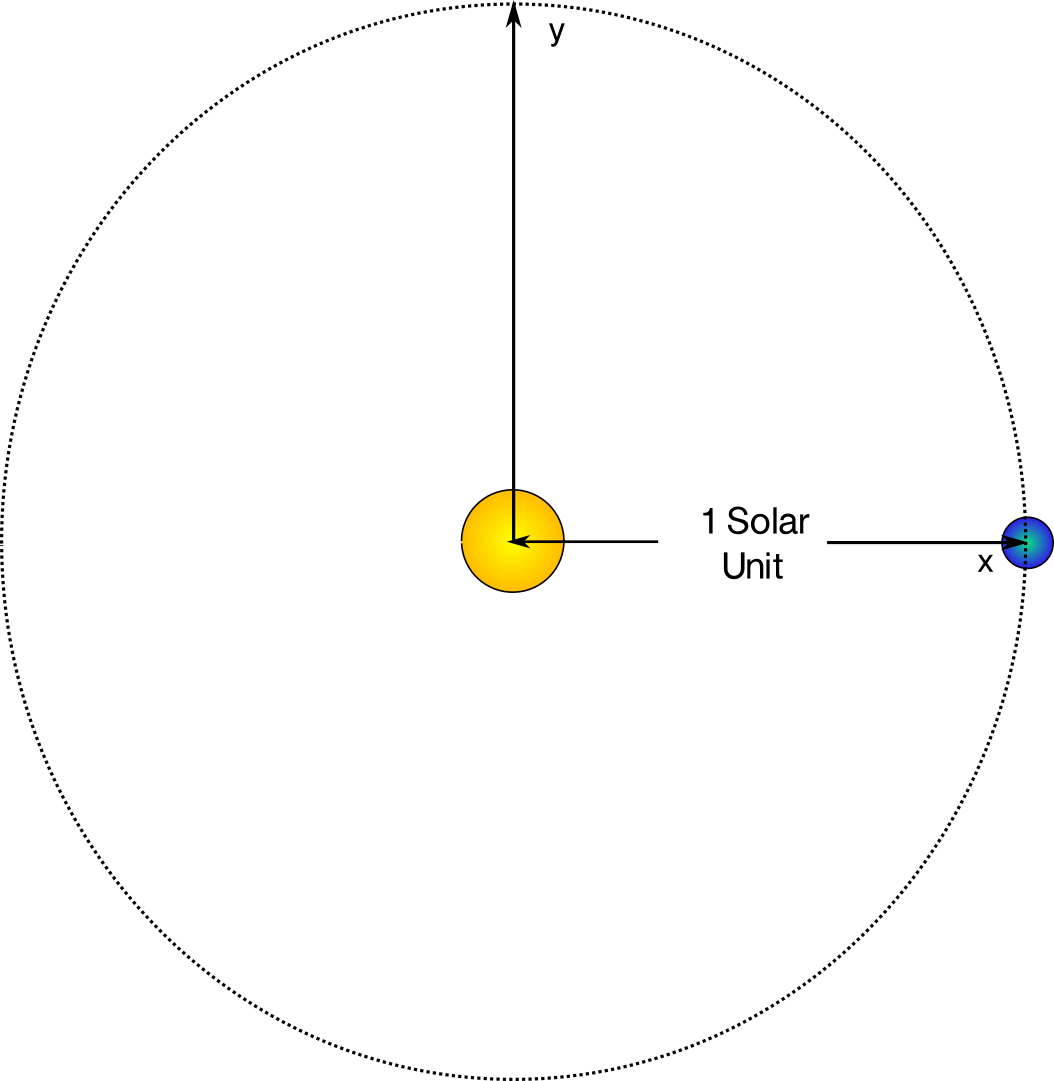
\includegraphics[width=20em]{angles/img/simpleSolarSystem}
  \end{center}

  \begin{subproblem}
  \item What distance does the earth traverse in one year?
    \vfill
  \item What distance does the earth traverse in two years?
    \vfill
  \item What distance does the earth traverse in ten years?
    \vfill
  \item What is the largest value that the $x$-coordinate can be?
    What is the smallest value that the $x$-coordinate can be?
    What is the largest value that the $y$-coordinate can be?
    What is the smallest value that the $y$-coordinate can be?
    \vfill
  \end{subproblem}

\end{problem}


\actTitle{Motion Around a Circle}
\begin{problem}
  \item An angle is in the second quadrant, and the sine of the angle is 0.2.
    Determine the cosine and tangent of the angle.
  \begin{subproblem}
    \item Make a sketch of the unit circle and place an angle somewhere in the second quadrant.
    Mark the point on the edge of the circle, $(x,y)$.
    \vfill

    \item Will the cosine be positive or negative? (Explain how you came to that conclusion.)
      Do the same for the tangent.
      \vfill

    \item Determine the cosine of the angle using the Pythagorean relationship between the sine
        and the cosine.
        \vfill

    \item Determine the tangent of the angle using the definition of the tangent.
      \vfill
  \end{subproblem}

  \clearpage

  \item A turtle moves around the edge of a circle of radius 1 meter.
  \begin{subproblem}
    \item After the turtle moves a distance of 2m what is its position?
      What quadrant is the point in?
      \sideNote{Make a sketch of the unit circle first and estimate its location.}
      \vfill
    \item After the turtle moves a distance of 4m what is its position?
      What quadrant is the point in?
      \sideNote{Make a sketch of the unit circle first and estimate its location.}
      \vfill
    \item After the turtle moves a distance of 6m what is its position?
      What quadrant is the point in?
      \sideNote{Make a sketch of the unit circle first and estimate its location.}
      \vfill
  \end{subproblem}

  \clearpage

  \item A turtle moves around the edge of a circle of radius 1 meter.
    \begin{subproblem}
      \item After it moves a distance of $\frac{\pi}{2}$ meters where is it on the circle?
      \sideNote{Make a rough sketch of the circle and indicate its position.}
      \vfill
      \item After it moves a distance of $\pi$ meters where is it on the circle?
      \vfill
      \item After it moves a distance of $\frac{3\pi}{2}$ meters where is it on the circle?
      \sideNote{Make a rough sketch of the circle and indicate its position.}
      \vfill
      \item After it moves a distance of $2\pi$ meters where is it on the circle?
      \vfill
      \item After it moves a distance of $5\pi$ meters where is it on the circle?
      \sideNote{Make a rough sketch of the circle and indicate its position.}
      \vfill
    \end{subproblem}

\clearpage

\item A turtle moves around the edge of a circle of radius 1 meter.
  \begin{subproblem}
    \item After it moves a distance of $\frac{\pi}{4}$ meters where is it on the circle?
    \sideNote{Make a rough sketch of the circle and indicate its position.}
    \vfill
    \item As the turtle moves from a distance of 0 meters to $\frac{\pi}{2}$ meters
      what is happening to the value of its $x$ coordinate. What about its $y$ coordinate?
    \vfill
    \item As the turtle moves from a distance of $\frac{\pi}{2}$ meters to $\pi$ meters
      what is happening to the value of its $x$ coordinate. What about its $y$ coordinate?
    \vfill
    \item As the turtle moves from a distance of $\pi$ meters to $\frac{3\pi}{2}$ meters
      what is happening to the value of its $x$ coordinate. What about its $y$ coordinate?
    \vfill
    \item As the turtle moves from a distance of $\frac{3\pi}{2}$ meters to $2\pi$ meters
      what is happening to the value of its $x$ coordinate. What about its $y$ coordinate?
    \vfill
  \end{subproblem}

\clearpage

\item When viewed above the north pole of the Sun, the earth appears
  to move around the sun in a counter-clockwise direction. The path
  can be roughly approximated as a circle. It takes
  one year to make one revolution, and assume that the distance from
  the center of the sun to the earth is one solar unit. (See the image
  in the preclass activity.)
  \begin{subproblem}
    \item What angle (in radians) does the earth make from the $x$-axis after 3
      months?
      %\vspace{1em}
      \vfill
    \item What angle (in radians) does the earth make from the $x$-axis after 6
      months?
      %\vspace{1em}
      \vfill
    \item Make a rough sketch of the earth's $y$ position as a
      function of the angle.

      \begin{tikzpicture}[y=2cm, x=2.7cm,font=\sffamily]
          % bounds
          \def\lowX{-0.5}
          \pgfmathtruncatemacro\startX{round(0.5+\lowX)}
          \pgfmathsetmacro\nextXValue{int(\startX+1)}
          \def\highX{5}
          \def\lowY{-1.25}
          \def\highY{1.25}
          \pgfmathsetmacro\nextYValue{int(\lowY+1)}
          % ticks
          \draw[step = 1, gray, very thin,dashed,opacity=0.85] (0, \lowY) grid ( \highX,\highY);
          % axis
          \draw[thick,->] (0,0) -- coordinate (x axis mid) (\highX,0) node[anchor = north west] {$\theta$};
          \draw[thick,->] (0,\lowY) -- coordinate (y axis mid) (0,\highY) node[anchor = north east] {$y$};

          \draw (1pt, 1) -- (-1pt, 1) node[yshift=-6,xshift=-1,anchor=east] { 1};
          \draw (1pt,-1) -- (-1pt,-1) node[yshift=-6,xshift=-1,anchor=east] {-1};

          \draw (1,1pt) -- (1,-1pt) node[yshift=-1,xshift=-1,anchor=north east] {$\frac{ \pi}{2}$};
          \draw (3,1pt) -- (3,-1pt) node[yshift=-1,xshift=-1,anchor=north east] {$\frac{3\pi}{2}$};
          \draw (5,1pt) -- (5,-1pt) node[yshift=-1,xshift=-1,anchor=north east] {$\frac{5\pi}{2}$};
          \draw (2,1pt) -- (2,-1pt) node[yshift=-1,xshift=-1,anchor=north east] {$\pi$};
          \draw (4,1pt) -- (4,-1pt) node[yshift=-1,xshift=-1,anchor=north east] {$2\pi$};
          \draw (2.5,1.3) node [anchor=south] {$Y$ Coordinate of the Earth};
        \end{tikzpicture}

    \item Make a rough sketch of the earth's $x$ position as a
      function of the angle.

      \begin{tikzpicture}[y=2cm, x=2.7cm,font=\sffamily]
          % bounds
          \def\lowX{-0.5}
          \pgfmathtruncatemacro\startX{round(0.5+\lowX)}
          \pgfmathsetmacro\nextXValue{int(\startX+1)}
          \def\highX{5}
          \def\lowY{-1.25}
          \def\highY{1.25}
          \pgfmathsetmacro\nextYValue{int(\lowY+1)}
          % ticks
          \draw[step = 1, gray, very thin,dashed,opacity=0.85] (0, \lowY) grid ( \highX,\highY);
          % axis
          \draw[thick,->] (0,0) -- coordinate (x axis mid) (\highX,0) node[anchor = north west] {$\theta$};
          \draw[thick,->] (0,\lowY) -- coordinate (y axis mid) (0,\highY) node[anchor = north east] {$x$};

          \draw (1pt, 1) -- (-1pt, 1) node[yshift=-6,xshift=-1,anchor=east] { 1};
          \draw (1pt,-1) -- (-1pt,-1) node[yshift=-6,xshift=-1,anchor=east] {-1};

          \draw (1,1pt) -- (1,-1pt) node[yshift=-1,xshift=-1,anchor=north east] {$\frac{ \pi}{2}$};
          \draw (3,1pt) -- (3,-1pt) node[yshift=-1,xshift=-1,anchor=north east] {$\frac{3\pi}{2}$};
          \draw (5,1pt) -- (5,-1pt) node[yshift=-1,xshift=-1,anchor=north east] {$\frac{5\pi}{2}$};
          \draw (2,1pt) -- (2,-1pt) node[yshift=-1,xshift=-1,anchor=north east] {$\pi$};
          \draw (4,1pt) -- (4,-1pt) node[yshift=-1,xshift=-1,anchor=north east] {$2\pi$};
          \draw (2.5,1.3) node [anchor=south] {$X$ Coordinate of the Earth};
        \end{tikzpicture}

  \end{subproblem}

  \clearpage

\item At the annual Plainfield $500\pi$ race a tractor will make 250 laps
  around a circular track. The track has a radius of 1 km. A single
  tractor will make a trial run by going around the track at 1 km per
  hour. (It is not a very fast race.) The car starts on the point
  furthest East and is initially moving to the North.

%      \scalebox{0.3}{%% Creator: Matplotlib, PGF backend
%%
%% To include the figure in your LaTeX document, write
%%   \input{<filename>.pgf}
%%
%% Make sure the required packages are loaded in your preamble
%%   \usepackage{pgf}
%%
%% Figures using additional raster images can only be included by \input if
%% they are in the same directory as the main LaTeX file. For loading figures
%% from other directories you can use the `import` package
%%   \usepackage{import}
%% and then include the figures with
%%   \import{<path to file>}{<filename>.pgf}
%%
%% Matplotlib used the following preamble
%%   \usepackage{fontspec}
%%   \setmainfont{Bitstream Vera Serif}
%%   \setsansfont{Bitstream Vera Sans}
%%   \setmonofont{Bitstream Vera Sans Mono}
%%
\begingroup%
\makeatletter%
\begin{pgfpicture}%
\pgfpathrectangle{\pgfpointorigin}{\pgfqpoint{8.000000in}{6.000000in}}%
\pgfusepath{use as bounding box, clip}%
\begin{pgfscope}%
\pgfsetbuttcap%
\pgfsetmiterjoin%
\definecolor{currentfill}{rgb}{1.000000,1.000000,1.000000}%
\pgfsetfillcolor{currentfill}%
\pgfsetlinewidth{0.000000pt}%
\definecolor{currentstroke}{rgb}{1.000000,1.000000,1.000000}%
\pgfsetstrokecolor{currentstroke}%
\pgfsetdash{}{0pt}%
\pgfpathmoveto{\pgfqpoint{0.000000in}{0.000000in}}%
\pgfpathlineto{\pgfqpoint{8.000000in}{0.000000in}}%
\pgfpathlineto{\pgfqpoint{8.000000in}{6.000000in}}%
\pgfpathlineto{\pgfqpoint{0.000000in}{6.000000in}}%
\pgfpathclose%
\pgfusepath{fill}%
\end{pgfscope}%
\begin{pgfscope}%
\pgfsetbuttcap%
\pgfsetmiterjoin%
\definecolor{currentfill}{rgb}{1.000000,1.000000,1.000000}%
\pgfsetfillcolor{currentfill}%
\pgfsetlinewidth{0.000000pt}%
\definecolor{currentstroke}{rgb}{0.000000,0.000000,0.000000}%
\pgfsetstrokecolor{currentstroke}%
\pgfsetstrokeopacity{0.000000}%
\pgfsetdash{}{0pt}%
\pgfpathmoveto{\pgfqpoint{1.000000in}{0.600000in}}%
\pgfpathlineto{\pgfqpoint{7.200000in}{0.600000in}}%
\pgfpathlineto{\pgfqpoint{7.200000in}{5.400000in}}%
\pgfpathlineto{\pgfqpoint{1.000000in}{5.400000in}}%
\pgfpathclose%
\pgfusepath{fill}%
\end{pgfscope}%
\begin{pgfscope}%
\pgfpathrectangle{\pgfqpoint{1.000000in}{0.600000in}}{\pgfqpoint{6.200000in}{4.800000in}} %
\pgfusepath{clip}%
\pgfsetbuttcap%
\pgfsetmiterjoin%
\definecolor{currentfill}{rgb}{0.000000,0.000000,0.000000}%
\pgfsetfillcolor{currentfill}%
\pgfsetlinewidth{1.003750pt}%
\definecolor{currentstroke}{rgb}{0.000000,0.000000,0.000000}%
\pgfsetstrokecolor{currentstroke}%
\pgfsetdash{}{0pt}%
\pgfpathmoveto{\pgfqpoint{5.797056in}{4.649056in}}%
\pgfpathcurveto{\pgfqpoint{5.809786in}{4.649056in}}{\pgfqpoint{5.821996in}{4.654114in}}{\pgfqpoint{5.830997in}{4.663115in}}%
\pgfpathcurveto{\pgfqpoint{5.839999in}{4.672116in}}{\pgfqpoint{5.845056in}{4.684327in}}{\pgfqpoint{5.845056in}{4.697056in}}%
\pgfpathcurveto{\pgfqpoint{5.845056in}{4.709786in}}{\pgfqpoint{5.839999in}{4.721996in}}{\pgfqpoint{5.830997in}{4.730997in}}%
\pgfpathcurveto{\pgfqpoint{5.821996in}{4.739999in}}{\pgfqpoint{5.809786in}{4.745056in}}{\pgfqpoint{5.797056in}{4.745056in}}%
\pgfpathcurveto{\pgfqpoint{5.784327in}{4.745056in}}{\pgfqpoint{5.772116in}{4.739999in}}{\pgfqpoint{5.763115in}{4.730997in}}%
\pgfpathcurveto{\pgfqpoint{5.754114in}{4.721996in}}{\pgfqpoint{5.749056in}{4.709786in}}{\pgfqpoint{5.749056in}{4.697056in}}%
\pgfpathcurveto{\pgfqpoint{5.749056in}{4.684327in}}{\pgfqpoint{5.754114in}{4.672116in}}{\pgfqpoint{5.763115in}{4.663115in}}%
\pgfpathcurveto{\pgfqpoint{5.772116in}{4.654114in}}{\pgfqpoint{5.784327in}{4.649056in}}{\pgfqpoint{5.797056in}{4.649056in}}%
\pgfpathlineto{\pgfqpoint{5.797056in}{4.649056in}}%
\pgfusepath{stroke,fill}%
\end{pgfscope}%
\begin{pgfscope}%
\pgfpathrectangle{\pgfqpoint{1.000000in}{0.600000in}}{\pgfqpoint{6.200000in}{4.800000in}} %
\pgfusepath{clip}%
\pgfsetrectcap%
\pgfsetroundjoin%
\pgfsetlinewidth{2.007500pt}%
\definecolor{currentstroke}{rgb}{0.000000,0.000000,0.000000}%
\pgfsetstrokecolor{currentstroke}%
\pgfsetdash{}{0pt}%
\pgfpathmoveto{\pgfqpoint{6.500000in}{3.000000in}}%
\pgfpathlineto{\pgfqpoint{6.498816in}{3.075386in}}%
\pgfpathlineto{\pgfqpoint{6.495264in}{3.150697in}}%
\pgfpathlineto{\pgfqpoint{6.489349in}{3.225860in}}%
\pgfpathlineto{\pgfqpoint{6.481075in}{3.300800in}}%
\pgfpathlineto{\pgfqpoint{6.470452in}{3.375443in}}%
\pgfpathlineto{\pgfqpoint{6.457489in}{3.449715in}}%
\pgfpathlineto{\pgfqpoint{6.442200in}{3.523544in}}%
\pgfpathlineto{\pgfqpoint{6.424600in}{3.596856in}}%
\pgfpathlineto{\pgfqpoint{6.404705in}{3.669579in}}%
\pgfpathlineto{\pgfqpoint{6.382536in}{3.741641in}}%
\pgfpathlineto{\pgfqpoint{6.358114in}{3.812971in}}%
\pgfpathlineto{\pgfqpoint{6.331464in}{3.883499in}}%
\pgfpathlineto{\pgfqpoint{6.302611in}{3.953155in}}%
\pgfpathlineto{\pgfqpoint{6.271585in}{4.021870in}}%
\pgfpathlineto{\pgfqpoint{6.238416in}{4.089577in}}%
\pgfpathlineto{\pgfqpoint{6.203136in}{4.156209in}}%
\pgfpathlineto{\pgfqpoint{6.165781in}{4.221699in}}%
\pgfpathlineto{\pgfqpoint{6.126387in}{4.285984in}}%
\pgfpathlineto{\pgfqpoint{6.084993in}{4.349000in}}%
\pgfpathlineto{\pgfqpoint{6.041641in}{4.410685in}}%
\pgfpathlineto{\pgfqpoint{5.996372in}{4.470977in}}%
\pgfpathlineto{\pgfqpoint{5.949232in}{4.529818in}}%
\pgfpathlineto{\pgfqpoint{5.900267in}{4.587148in}}%
\pgfpathlineto{\pgfqpoint{5.849525in}{4.642913in}}%
\pgfpathlineto{\pgfqpoint{5.797056in}{4.697056in}}%
\pgfpathlineto{\pgfqpoint{5.742913in}{4.749525in}}%
\pgfpathlineto{\pgfqpoint{5.687148in}{4.800267in}}%
\pgfpathlineto{\pgfqpoint{5.629818in}{4.849232in}}%
\pgfpathlineto{\pgfqpoint{5.570977in}{4.896372in}}%
\pgfpathlineto{\pgfqpoint{5.510685in}{4.941641in}}%
\pgfpathlineto{\pgfqpoint{5.449000in}{4.984993in}}%
\pgfpathlineto{\pgfqpoint{5.385984in}{5.026387in}}%
\pgfpathlineto{\pgfqpoint{5.321699in}{5.065781in}}%
\pgfpathlineto{\pgfqpoint{5.256209in}{5.103136in}}%
\pgfpathlineto{\pgfqpoint{5.189577in}{5.138416in}}%
\pgfpathlineto{\pgfqpoint{5.121870in}{5.171585in}}%
\pgfpathlineto{\pgfqpoint{5.053155in}{5.202611in}}%
\pgfpathlineto{\pgfqpoint{4.983499in}{5.231464in}}%
\pgfpathlineto{\pgfqpoint{4.912971in}{5.258114in}}%
\pgfpathlineto{\pgfqpoint{4.841641in}{5.282536in}}%
\pgfpathlineto{\pgfqpoint{4.769579in}{5.304705in}}%
\pgfpathlineto{\pgfqpoint{4.696856in}{5.324600in}}%
\pgfpathlineto{\pgfqpoint{4.623544in}{5.342200in}}%
\pgfpathlineto{\pgfqpoint{4.549715in}{5.357489in}}%
\pgfpathlineto{\pgfqpoint{4.475443in}{5.370452in}}%
\pgfpathlineto{\pgfqpoint{4.400800in}{5.381075in}}%
\pgfpathlineto{\pgfqpoint{4.325860in}{5.389349in}}%
\pgfpathlineto{\pgfqpoint{4.250697in}{5.395264in}}%
\pgfpathlineto{\pgfqpoint{4.175386in}{5.398816in}}%
\pgfpathlineto{\pgfqpoint{4.100000in}{5.400000in}}%
\pgfpathlineto{\pgfqpoint{4.024614in}{5.398816in}}%
\pgfpathlineto{\pgfqpoint{3.949303in}{5.395264in}}%
\pgfpathlineto{\pgfqpoint{3.874140in}{5.389349in}}%
\pgfpathlineto{\pgfqpoint{3.799200in}{5.381075in}}%
\pgfpathlineto{\pgfqpoint{3.724557in}{5.370452in}}%
\pgfpathlineto{\pgfqpoint{3.650285in}{5.357489in}}%
\pgfpathlineto{\pgfqpoint{3.576456in}{5.342200in}}%
\pgfpathlineto{\pgfqpoint{3.503144in}{5.324600in}}%
\pgfpathlineto{\pgfqpoint{3.430421in}{5.304705in}}%
\pgfpathlineto{\pgfqpoint{3.358359in}{5.282536in}}%
\pgfpathlineto{\pgfqpoint{3.287029in}{5.258114in}}%
\pgfpathlineto{\pgfqpoint{3.216501in}{5.231464in}}%
\pgfpathlineto{\pgfqpoint{3.146845in}{5.202611in}}%
\pgfpathlineto{\pgfqpoint{3.078130in}{5.171585in}}%
\pgfpathlineto{\pgfqpoint{3.010423in}{5.138416in}}%
\pgfpathlineto{\pgfqpoint{2.943791in}{5.103136in}}%
\pgfpathlineto{\pgfqpoint{2.878301in}{5.065781in}}%
\pgfpathlineto{\pgfqpoint{2.814016in}{5.026387in}}%
\pgfpathlineto{\pgfqpoint{2.751000in}{4.984993in}}%
\pgfpathlineto{\pgfqpoint{2.689315in}{4.941641in}}%
\pgfpathlineto{\pgfqpoint{2.629023in}{4.896372in}}%
\pgfpathlineto{\pgfqpoint{2.570182in}{4.849232in}}%
\pgfpathlineto{\pgfqpoint{2.512852in}{4.800267in}}%
\pgfpathlineto{\pgfqpoint{2.457087in}{4.749525in}}%
\pgfpathlineto{\pgfqpoint{2.402944in}{4.697056in}}%
\pgfpathlineto{\pgfqpoint{2.350475in}{4.642913in}}%
\pgfpathlineto{\pgfqpoint{2.299733in}{4.587148in}}%
\pgfpathlineto{\pgfqpoint{2.250768in}{4.529818in}}%
\pgfpathlineto{\pgfqpoint{2.203628in}{4.470977in}}%
\pgfpathlineto{\pgfqpoint{2.158359in}{4.410685in}}%
\pgfpathlineto{\pgfqpoint{2.115007in}{4.349000in}}%
\pgfpathlineto{\pgfqpoint{2.073613in}{4.285984in}}%
\pgfpathlineto{\pgfqpoint{2.034219in}{4.221699in}}%
\pgfpathlineto{\pgfqpoint{1.996864in}{4.156209in}}%
\pgfpathlineto{\pgfqpoint{1.961584in}{4.089577in}}%
\pgfpathlineto{\pgfqpoint{1.928415in}{4.021870in}}%
\pgfpathlineto{\pgfqpoint{1.897389in}{3.953155in}}%
\pgfpathlineto{\pgfqpoint{1.868536in}{3.883499in}}%
\pgfpathlineto{\pgfqpoint{1.841886in}{3.812971in}}%
\pgfpathlineto{\pgfqpoint{1.817464in}{3.741641in}}%
\pgfpathlineto{\pgfqpoint{1.795295in}{3.669579in}}%
\pgfpathlineto{\pgfqpoint{1.775400in}{3.596856in}}%
\pgfpathlineto{\pgfqpoint{1.757800in}{3.523544in}}%
\pgfpathlineto{\pgfqpoint{1.742511in}{3.449715in}}%
\pgfpathlineto{\pgfqpoint{1.729548in}{3.375443in}}%
\pgfpathlineto{\pgfqpoint{1.718925in}{3.300800in}}%
\pgfpathlineto{\pgfqpoint{1.710651in}{3.225860in}}%
\pgfpathlineto{\pgfqpoint{1.704736in}{3.150697in}}%
\pgfpathlineto{\pgfqpoint{1.701184in}{3.075386in}}%
\pgfpathlineto{\pgfqpoint{1.700000in}{3.000000in}}%
\pgfpathlineto{\pgfqpoint{1.701184in}{2.924614in}}%
\pgfpathlineto{\pgfqpoint{1.704736in}{2.849303in}}%
\pgfpathlineto{\pgfqpoint{1.710651in}{2.774140in}}%
\pgfpathlineto{\pgfqpoint{1.718925in}{2.699200in}}%
\pgfpathlineto{\pgfqpoint{1.729548in}{2.624557in}}%
\pgfpathlineto{\pgfqpoint{1.742511in}{2.550285in}}%
\pgfpathlineto{\pgfqpoint{1.757800in}{2.476456in}}%
\pgfpathlineto{\pgfqpoint{1.775400in}{2.403144in}}%
\pgfpathlineto{\pgfqpoint{1.795295in}{2.330421in}}%
\pgfpathlineto{\pgfqpoint{1.817464in}{2.258359in}}%
\pgfpathlineto{\pgfqpoint{1.841886in}{2.187029in}}%
\pgfpathlineto{\pgfqpoint{1.868536in}{2.116501in}}%
\pgfpathlineto{\pgfqpoint{1.897389in}{2.046845in}}%
\pgfpathlineto{\pgfqpoint{1.928415in}{1.978130in}}%
\pgfpathlineto{\pgfqpoint{1.961584in}{1.910423in}}%
\pgfpathlineto{\pgfqpoint{1.996864in}{1.843791in}}%
\pgfpathlineto{\pgfqpoint{2.034219in}{1.778301in}}%
\pgfpathlineto{\pgfqpoint{2.073613in}{1.714016in}}%
\pgfpathlineto{\pgfqpoint{2.115007in}{1.651000in}}%
\pgfpathlineto{\pgfqpoint{2.158359in}{1.589315in}}%
\pgfpathlineto{\pgfqpoint{2.203628in}{1.529023in}}%
\pgfpathlineto{\pgfqpoint{2.250768in}{1.470182in}}%
\pgfpathlineto{\pgfqpoint{2.299733in}{1.412852in}}%
\pgfpathlineto{\pgfqpoint{2.350475in}{1.357087in}}%
\pgfpathlineto{\pgfqpoint{2.402944in}{1.302944in}}%
\pgfpathlineto{\pgfqpoint{2.457087in}{1.250475in}}%
\pgfpathlineto{\pgfqpoint{2.512852in}{1.199733in}}%
\pgfpathlineto{\pgfqpoint{2.570182in}{1.150768in}}%
\pgfpathlineto{\pgfqpoint{2.629023in}{1.103628in}}%
\pgfpathlineto{\pgfqpoint{2.689315in}{1.058359in}}%
\pgfpathlineto{\pgfqpoint{2.751000in}{1.015007in}}%
\pgfpathlineto{\pgfqpoint{2.814016in}{0.973613in}}%
\pgfpathlineto{\pgfqpoint{2.878301in}{0.934219in}}%
\pgfpathlineto{\pgfqpoint{2.943791in}{0.896864in}}%
\pgfpathlineto{\pgfqpoint{3.010423in}{0.861584in}}%
\pgfpathlineto{\pgfqpoint{3.078130in}{0.828415in}}%
\pgfpathlineto{\pgfqpoint{3.146845in}{0.797389in}}%
\pgfpathlineto{\pgfqpoint{3.216501in}{0.768536in}}%
\pgfpathlineto{\pgfqpoint{3.287029in}{0.741886in}}%
\pgfpathlineto{\pgfqpoint{3.358359in}{0.717464in}}%
\pgfpathlineto{\pgfqpoint{3.430421in}{0.695295in}}%
\pgfpathlineto{\pgfqpoint{3.503144in}{0.675400in}}%
\pgfpathlineto{\pgfqpoint{3.576456in}{0.657800in}}%
\pgfpathlineto{\pgfqpoint{3.650285in}{0.642511in}}%
\pgfpathlineto{\pgfqpoint{3.724557in}{0.629548in}}%
\pgfpathlineto{\pgfqpoint{3.799200in}{0.618925in}}%
\pgfpathlineto{\pgfqpoint{3.874140in}{0.610651in}}%
\pgfpathlineto{\pgfqpoint{3.949303in}{0.604736in}}%
\pgfpathlineto{\pgfqpoint{4.024614in}{0.601184in}}%
\pgfpathlineto{\pgfqpoint{4.100000in}{0.600000in}}%
\pgfpathlineto{\pgfqpoint{4.175386in}{0.601184in}}%
\pgfpathlineto{\pgfqpoint{4.250697in}{0.604736in}}%
\pgfpathlineto{\pgfqpoint{4.325860in}{0.610651in}}%
\pgfpathlineto{\pgfqpoint{4.400800in}{0.618925in}}%
\pgfpathlineto{\pgfqpoint{4.475443in}{0.629548in}}%
\pgfpathlineto{\pgfqpoint{4.549715in}{0.642511in}}%
\pgfpathlineto{\pgfqpoint{4.623544in}{0.657800in}}%
\pgfpathlineto{\pgfqpoint{4.696856in}{0.675400in}}%
\pgfpathlineto{\pgfqpoint{4.769579in}{0.695295in}}%
\pgfpathlineto{\pgfqpoint{4.841641in}{0.717464in}}%
\pgfpathlineto{\pgfqpoint{4.912971in}{0.741886in}}%
\pgfpathlineto{\pgfqpoint{4.983499in}{0.768536in}}%
\pgfpathlineto{\pgfqpoint{5.053155in}{0.797389in}}%
\pgfpathlineto{\pgfqpoint{5.121870in}{0.828415in}}%
\pgfpathlineto{\pgfqpoint{5.189577in}{0.861584in}}%
\pgfpathlineto{\pgfqpoint{5.256209in}{0.896864in}}%
\pgfpathlineto{\pgfqpoint{5.321699in}{0.934219in}}%
\pgfpathlineto{\pgfqpoint{5.385984in}{0.973613in}}%
\pgfpathlineto{\pgfqpoint{5.449000in}{1.015007in}}%
\pgfpathlineto{\pgfqpoint{5.510685in}{1.058359in}}%
\pgfpathlineto{\pgfqpoint{5.570977in}{1.103628in}}%
\pgfpathlineto{\pgfqpoint{5.629818in}{1.150768in}}%
\pgfpathlineto{\pgfqpoint{5.687148in}{1.199733in}}%
\pgfpathlineto{\pgfqpoint{5.742913in}{1.250475in}}%
\pgfpathlineto{\pgfqpoint{5.797056in}{1.302944in}}%
\pgfpathlineto{\pgfqpoint{5.849525in}{1.357087in}}%
\pgfpathlineto{\pgfqpoint{5.900267in}{1.412852in}}%
\pgfpathlineto{\pgfqpoint{5.949232in}{1.470182in}}%
\pgfpathlineto{\pgfqpoint{5.996372in}{1.529023in}}%
\pgfpathlineto{\pgfqpoint{6.041641in}{1.589315in}}%
\pgfpathlineto{\pgfqpoint{6.084993in}{1.651000in}}%
\pgfpathlineto{\pgfqpoint{6.126387in}{1.714016in}}%
\pgfpathlineto{\pgfqpoint{6.165781in}{1.778301in}}%
\pgfpathlineto{\pgfqpoint{6.203136in}{1.843791in}}%
\pgfpathlineto{\pgfqpoint{6.238416in}{1.910423in}}%
\pgfpathlineto{\pgfqpoint{6.271585in}{1.978130in}}%
\pgfpathlineto{\pgfqpoint{6.302611in}{2.046845in}}%
\pgfpathlineto{\pgfqpoint{6.331464in}{2.116501in}}%
\pgfpathlineto{\pgfqpoint{6.358114in}{2.187029in}}%
\pgfpathlineto{\pgfqpoint{6.382536in}{2.258359in}}%
\pgfpathlineto{\pgfqpoint{6.404705in}{2.330421in}}%
\pgfpathlineto{\pgfqpoint{6.424600in}{2.403144in}}%
\pgfpathlineto{\pgfqpoint{6.442200in}{2.476456in}}%
\pgfpathlineto{\pgfqpoint{6.457489in}{2.550285in}}%
\pgfpathlineto{\pgfqpoint{6.470452in}{2.624557in}}%
\pgfpathlineto{\pgfqpoint{6.481075in}{2.699200in}}%
\pgfpathlineto{\pgfqpoint{6.489349in}{2.774140in}}%
\pgfpathlineto{\pgfqpoint{6.495264in}{2.849303in}}%
\pgfpathlineto{\pgfqpoint{6.498816in}{2.924614in}}%
\pgfpathlineto{\pgfqpoint{6.498816in}{2.924614in}}%
\pgfusepath{stroke}%
\end{pgfscope}%
\begin{pgfscope}%
\pgfpathrectangle{\pgfqpoint{1.000000in}{0.600000in}}{\pgfqpoint{6.200000in}{4.800000in}} %
\pgfusepath{clip}%
\pgfsetrectcap%
\pgfsetroundjoin%
\pgfsetlinewidth{2.007500pt}%
\definecolor{currentstroke}{rgb}{0.000000,0.000000,0.000000}%
\pgfsetstrokecolor{currentstroke}%
\pgfsetdash{}{0pt}%
\pgfpathmoveto{\pgfqpoint{4.100000in}{3.000000in}}%
\pgfpathlineto{\pgfqpoint{5.797056in}{4.697056in}}%
\pgfusepath{stroke}%
\end{pgfscope}%
\begin{pgfscope}%
\pgfsetrectcap%
\pgfsetmiterjoin%
\pgfsetlinewidth{0.000000pt}%
\definecolor{currentstroke}{rgb}{0.000000,0.000000,0.000000}%
\pgfsetstrokecolor{currentstroke}%
\pgfsetstrokeopacity{0.000000}%
\pgfsetdash{}{0pt}%
\pgfpathmoveto{\pgfqpoint{1.000000in}{5.400000in}}%
\pgfpathlineto{\pgfqpoint{7.200000in}{5.400000in}}%
\pgfusepath{}%
\end{pgfscope}%
\begin{pgfscope}%
\pgfsetrectcap%
\pgfsetmiterjoin%
\pgfsetlinewidth{0.000000pt}%
\definecolor{currentstroke}{rgb}{0.000000,0.000000,0.000000}%
\pgfsetstrokecolor{currentstroke}%
\pgfsetstrokeopacity{0.000000}%
\pgfsetdash{}{0pt}%
\pgfpathmoveto{\pgfqpoint{7.200000in}{0.600000in}}%
\pgfpathlineto{\pgfqpoint{7.200000in}{5.400000in}}%
\pgfusepath{}%
\end{pgfscope}%
\begin{pgfscope}%
\pgfsetrectcap%
\pgfsetmiterjoin%
\pgfsetlinewidth{1.003750pt}%
\definecolor{currentstroke}{rgb}{0.000000,0.000000,0.000000}%
\pgfsetstrokecolor{currentstroke}%
\pgfsetdash{}{0pt}%
\pgfpathmoveto{\pgfqpoint{1.000000in}{3.000000in}}%
\pgfpathlineto{\pgfqpoint{7.200000in}{3.000000in}}%
\pgfusepath{stroke}%
\end{pgfscope}%
\begin{pgfscope}%
\pgfsetrectcap%
\pgfsetmiterjoin%
\pgfsetlinewidth{1.003750pt}%
\definecolor{currentstroke}{rgb}{0.000000,0.000000,0.000000}%
\pgfsetstrokecolor{currentstroke}%
\pgfsetdash{}{0pt}%
\pgfpathmoveto{\pgfqpoint{4.100000in}{0.600000in}}%
\pgfpathlineto{\pgfqpoint{4.100000in}{5.400000in}}%
\pgfusepath{stroke}%
\end{pgfscope}%
\begin{pgfscope}%
\pgfsetbuttcap%
\pgfsetroundjoin%
\pgfsetlinewidth{0.501875pt}%
\definecolor{currentstroke}{rgb}{0.000000,0.000000,0.000000}%
\pgfsetstrokecolor{currentstroke}%
\pgfsetdash{{1.000000pt}{3.000000pt}}{0.000000pt}%
\pgfpathmoveto{\pgfqpoint{1.700000in}{0.600000in}}%
\pgfpathlineto{\pgfqpoint{1.700000in}{5.400000in}}%
\pgfusepath{stroke}%
\end{pgfscope}%
\begin{pgfscope}%
\pgfsetbuttcap%
\pgfsetroundjoin%
\definecolor{currentfill}{rgb}{0.000000,0.000000,0.000000}%
\pgfsetfillcolor{currentfill}%
\pgfsetlinewidth{0.501875pt}%
\definecolor{currentstroke}{rgb}{0.000000,0.000000,0.000000}%
\pgfsetstrokecolor{currentstroke}%
\pgfsetdash{}{0pt}%
\pgfsys@defobject{currentmarker}{\pgfqpoint{0.000000in}{0.000000in}}{\pgfqpoint{0.000000in}{0.055556in}}{%
\pgfpathmoveto{\pgfqpoint{0.000000in}{0.000000in}}%
\pgfpathlineto{\pgfqpoint{0.000000in}{0.055556in}}%
\pgfusepath{stroke,fill}%
}%
\begin{pgfscope}%
\pgfsys@transformshift{1.700000in}{3.000000in}%
\pgfsys@useobject{currentmarker}{}%
\end{pgfscope}%
\end{pgfscope}%
\begin{pgfscope}%
\pgftext[x=1.700000in,y=2.944444in,,top]{\sffamily\fontsize{12.000000}{14.400000}\selectfont \(\displaystyle -1.0\)}%
\end{pgfscope}%
\begin{pgfscope}%
\pgfsetbuttcap%
\pgfsetroundjoin%
\pgfsetlinewidth{0.501875pt}%
\definecolor{currentstroke}{rgb}{0.000000,0.000000,0.000000}%
\pgfsetstrokecolor{currentstroke}%
\pgfsetdash{{1.000000pt}{3.000000pt}}{0.000000pt}%
\pgfpathmoveto{\pgfqpoint{2.900000in}{0.600000in}}%
\pgfpathlineto{\pgfqpoint{2.900000in}{5.400000in}}%
\pgfusepath{stroke}%
\end{pgfscope}%
\begin{pgfscope}%
\pgfsetbuttcap%
\pgfsetroundjoin%
\definecolor{currentfill}{rgb}{0.000000,0.000000,0.000000}%
\pgfsetfillcolor{currentfill}%
\pgfsetlinewidth{0.501875pt}%
\definecolor{currentstroke}{rgb}{0.000000,0.000000,0.000000}%
\pgfsetstrokecolor{currentstroke}%
\pgfsetdash{}{0pt}%
\pgfsys@defobject{currentmarker}{\pgfqpoint{0.000000in}{0.000000in}}{\pgfqpoint{0.000000in}{0.055556in}}{%
\pgfpathmoveto{\pgfqpoint{0.000000in}{0.000000in}}%
\pgfpathlineto{\pgfqpoint{0.000000in}{0.055556in}}%
\pgfusepath{stroke,fill}%
}%
\begin{pgfscope}%
\pgfsys@transformshift{2.900000in}{3.000000in}%
\pgfsys@useobject{currentmarker}{}%
\end{pgfscope}%
\end{pgfscope}%
\begin{pgfscope}%
\pgftext[x=2.900000in,y=2.944444in,,top]{\sffamily\fontsize{12.000000}{14.400000}\selectfont \(\displaystyle -0.5\)}%
\end{pgfscope}%
\begin{pgfscope}%
\pgfsetbuttcap%
\pgfsetroundjoin%
\pgfsetlinewidth{0.501875pt}%
\definecolor{currentstroke}{rgb}{0.000000,0.000000,0.000000}%
\pgfsetstrokecolor{currentstroke}%
\pgfsetdash{{1.000000pt}{3.000000pt}}{0.000000pt}%
\pgfpathmoveto{\pgfqpoint{4.100000in}{0.600000in}}%
\pgfpathlineto{\pgfqpoint{4.100000in}{5.400000in}}%
\pgfusepath{stroke}%
\end{pgfscope}%
\begin{pgfscope}%
\pgfsetbuttcap%
\pgfsetroundjoin%
\definecolor{currentfill}{rgb}{0.000000,0.000000,0.000000}%
\pgfsetfillcolor{currentfill}%
\pgfsetlinewidth{0.501875pt}%
\definecolor{currentstroke}{rgb}{0.000000,0.000000,0.000000}%
\pgfsetstrokecolor{currentstroke}%
\pgfsetdash{}{0pt}%
\pgfsys@defobject{currentmarker}{\pgfqpoint{0.000000in}{0.000000in}}{\pgfqpoint{0.000000in}{0.055556in}}{%
\pgfpathmoveto{\pgfqpoint{0.000000in}{0.000000in}}%
\pgfpathlineto{\pgfqpoint{0.000000in}{0.055556in}}%
\pgfusepath{stroke,fill}%
}%
\begin{pgfscope}%
\pgfsys@transformshift{4.100000in}{3.000000in}%
\pgfsys@useobject{currentmarker}{}%
\end{pgfscope}%
\end{pgfscope}%
\begin{pgfscope}%
\pgftext[x=4.100000in,y=2.944444in,,top]{\sffamily\fontsize{12.000000}{14.400000}\selectfont \(\displaystyle 0.0\)}%
\end{pgfscope}%
\begin{pgfscope}%
\pgfsetbuttcap%
\pgfsetroundjoin%
\pgfsetlinewidth{0.501875pt}%
\definecolor{currentstroke}{rgb}{0.000000,0.000000,0.000000}%
\pgfsetstrokecolor{currentstroke}%
\pgfsetdash{{1.000000pt}{3.000000pt}}{0.000000pt}%
\pgfpathmoveto{\pgfqpoint{5.300000in}{0.600000in}}%
\pgfpathlineto{\pgfqpoint{5.300000in}{5.400000in}}%
\pgfusepath{stroke}%
\end{pgfscope}%
\begin{pgfscope}%
\pgfsetbuttcap%
\pgfsetroundjoin%
\definecolor{currentfill}{rgb}{0.000000,0.000000,0.000000}%
\pgfsetfillcolor{currentfill}%
\pgfsetlinewidth{0.501875pt}%
\definecolor{currentstroke}{rgb}{0.000000,0.000000,0.000000}%
\pgfsetstrokecolor{currentstroke}%
\pgfsetdash{}{0pt}%
\pgfsys@defobject{currentmarker}{\pgfqpoint{0.000000in}{0.000000in}}{\pgfqpoint{0.000000in}{0.055556in}}{%
\pgfpathmoveto{\pgfqpoint{0.000000in}{0.000000in}}%
\pgfpathlineto{\pgfqpoint{0.000000in}{0.055556in}}%
\pgfusepath{stroke,fill}%
}%
\begin{pgfscope}%
\pgfsys@transformshift{5.300000in}{3.000000in}%
\pgfsys@useobject{currentmarker}{}%
\end{pgfscope}%
\end{pgfscope}%
\begin{pgfscope}%
\pgftext[x=5.300000in,y=2.944444in,,top]{\sffamily\fontsize{12.000000}{14.400000}\selectfont \(\displaystyle 0.5\)}%
\end{pgfscope}%
\begin{pgfscope}%
\pgfsetbuttcap%
\pgfsetroundjoin%
\pgfsetlinewidth{0.501875pt}%
\definecolor{currentstroke}{rgb}{0.000000,0.000000,0.000000}%
\pgfsetstrokecolor{currentstroke}%
\pgfsetdash{{1.000000pt}{3.000000pt}}{0.000000pt}%
\pgfpathmoveto{\pgfqpoint{6.500000in}{0.600000in}}%
\pgfpathlineto{\pgfqpoint{6.500000in}{5.400000in}}%
\pgfusepath{stroke}%
\end{pgfscope}%
\begin{pgfscope}%
\pgfsetbuttcap%
\pgfsetroundjoin%
\definecolor{currentfill}{rgb}{0.000000,0.000000,0.000000}%
\pgfsetfillcolor{currentfill}%
\pgfsetlinewidth{0.501875pt}%
\definecolor{currentstroke}{rgb}{0.000000,0.000000,0.000000}%
\pgfsetstrokecolor{currentstroke}%
\pgfsetdash{}{0pt}%
\pgfsys@defobject{currentmarker}{\pgfqpoint{0.000000in}{0.000000in}}{\pgfqpoint{0.000000in}{0.055556in}}{%
\pgfpathmoveto{\pgfqpoint{0.000000in}{0.000000in}}%
\pgfpathlineto{\pgfqpoint{0.000000in}{0.055556in}}%
\pgfusepath{stroke,fill}%
}%
\begin{pgfscope}%
\pgfsys@transformshift{6.500000in}{3.000000in}%
\pgfsys@useobject{currentmarker}{}%
\end{pgfscope}%
\end{pgfscope}%
\begin{pgfscope}%
\pgftext[x=6.500000in,y=2.944444in,,top]{\sffamily\fontsize{12.000000}{14.400000}\selectfont \(\displaystyle 1.0\)}%
\end{pgfscope}%
\begin{pgfscope}%
\pgftext[x=7.014000in,y=2.760000in,,top]{\sffamily\fontsize{12.000000}{14.400000}\selectfont x}%
\end{pgfscope}%
\begin{pgfscope}%
\pgfsetbuttcap%
\pgfsetroundjoin%
\pgfsetlinewidth{0.501875pt}%
\definecolor{currentstroke}{rgb}{0.000000,0.000000,0.000000}%
\pgfsetstrokecolor{currentstroke}%
\pgfsetdash{{1.000000pt}{3.000000pt}}{0.000000pt}%
\pgfpathmoveto{\pgfqpoint{1.000000in}{0.600000in}}%
\pgfpathlineto{\pgfqpoint{7.200000in}{0.600000in}}%
\pgfusepath{stroke}%
\end{pgfscope}%
\begin{pgfscope}%
\pgfsetbuttcap%
\pgfsetroundjoin%
\definecolor{currentfill}{rgb}{0.000000,0.000000,0.000000}%
\pgfsetfillcolor{currentfill}%
\pgfsetlinewidth{0.501875pt}%
\definecolor{currentstroke}{rgb}{0.000000,0.000000,0.000000}%
\pgfsetstrokecolor{currentstroke}%
\pgfsetdash{}{0pt}%
\pgfsys@defobject{currentmarker}{\pgfqpoint{0.000000in}{0.000000in}}{\pgfqpoint{0.055556in}{0.000000in}}{%
\pgfpathmoveto{\pgfqpoint{0.000000in}{0.000000in}}%
\pgfpathlineto{\pgfqpoint{0.055556in}{0.000000in}}%
\pgfusepath{stroke,fill}%
}%
\begin{pgfscope}%
\pgfsys@transformshift{4.100000in}{0.600000in}%
\pgfsys@useobject{currentmarker}{}%
\end{pgfscope}%
\end{pgfscope}%
\begin{pgfscope}%
\pgftext[x=4.044444in,y=0.600000in,right,]{\sffamily\fontsize{12.000000}{14.400000}\selectfont \(\displaystyle -1.0\)}%
\end{pgfscope}%
\begin{pgfscope}%
\pgfsetbuttcap%
\pgfsetroundjoin%
\pgfsetlinewidth{0.501875pt}%
\definecolor{currentstroke}{rgb}{0.000000,0.000000,0.000000}%
\pgfsetstrokecolor{currentstroke}%
\pgfsetdash{{1.000000pt}{3.000000pt}}{0.000000pt}%
\pgfpathmoveto{\pgfqpoint{1.000000in}{1.800000in}}%
\pgfpathlineto{\pgfqpoint{7.200000in}{1.800000in}}%
\pgfusepath{stroke}%
\end{pgfscope}%
\begin{pgfscope}%
\pgfsetbuttcap%
\pgfsetroundjoin%
\definecolor{currentfill}{rgb}{0.000000,0.000000,0.000000}%
\pgfsetfillcolor{currentfill}%
\pgfsetlinewidth{0.501875pt}%
\definecolor{currentstroke}{rgb}{0.000000,0.000000,0.000000}%
\pgfsetstrokecolor{currentstroke}%
\pgfsetdash{}{0pt}%
\pgfsys@defobject{currentmarker}{\pgfqpoint{0.000000in}{0.000000in}}{\pgfqpoint{0.055556in}{0.000000in}}{%
\pgfpathmoveto{\pgfqpoint{0.000000in}{0.000000in}}%
\pgfpathlineto{\pgfqpoint{0.055556in}{0.000000in}}%
\pgfusepath{stroke,fill}%
}%
\begin{pgfscope}%
\pgfsys@transformshift{4.100000in}{1.800000in}%
\pgfsys@useobject{currentmarker}{}%
\end{pgfscope}%
\end{pgfscope}%
\begin{pgfscope}%
\pgftext[x=4.044444in,y=1.800000in,right,]{\sffamily\fontsize{12.000000}{14.400000}\selectfont \(\displaystyle -0.5\)}%
\end{pgfscope}%
\begin{pgfscope}%
\pgfsetbuttcap%
\pgfsetroundjoin%
\pgfsetlinewidth{0.501875pt}%
\definecolor{currentstroke}{rgb}{0.000000,0.000000,0.000000}%
\pgfsetstrokecolor{currentstroke}%
\pgfsetdash{{1.000000pt}{3.000000pt}}{0.000000pt}%
\pgfpathmoveto{\pgfqpoint{1.000000in}{3.000000in}}%
\pgfpathlineto{\pgfqpoint{7.200000in}{3.000000in}}%
\pgfusepath{stroke}%
\end{pgfscope}%
\begin{pgfscope}%
\pgfsetbuttcap%
\pgfsetroundjoin%
\definecolor{currentfill}{rgb}{0.000000,0.000000,0.000000}%
\pgfsetfillcolor{currentfill}%
\pgfsetlinewidth{0.501875pt}%
\definecolor{currentstroke}{rgb}{0.000000,0.000000,0.000000}%
\pgfsetstrokecolor{currentstroke}%
\pgfsetdash{}{0pt}%
\pgfsys@defobject{currentmarker}{\pgfqpoint{0.000000in}{0.000000in}}{\pgfqpoint{0.055556in}{0.000000in}}{%
\pgfpathmoveto{\pgfqpoint{0.000000in}{0.000000in}}%
\pgfpathlineto{\pgfqpoint{0.055556in}{0.000000in}}%
\pgfusepath{stroke,fill}%
}%
\begin{pgfscope}%
\pgfsys@transformshift{4.100000in}{3.000000in}%
\pgfsys@useobject{currentmarker}{}%
\end{pgfscope}%
\end{pgfscope}%
\begin{pgfscope}%
\pgftext[x=4.044444in,y=3.000000in,right,]{\sffamily\fontsize{12.000000}{14.400000}\selectfont \(\displaystyle 0.0\)}%
\end{pgfscope}%
\begin{pgfscope}%
\pgfsetbuttcap%
\pgfsetroundjoin%
\pgfsetlinewidth{0.501875pt}%
\definecolor{currentstroke}{rgb}{0.000000,0.000000,0.000000}%
\pgfsetstrokecolor{currentstroke}%
\pgfsetdash{{1.000000pt}{3.000000pt}}{0.000000pt}%
\pgfpathmoveto{\pgfqpoint{1.000000in}{4.200000in}}%
\pgfpathlineto{\pgfqpoint{7.200000in}{4.200000in}}%
\pgfusepath{stroke}%
\end{pgfscope}%
\begin{pgfscope}%
\pgfsetbuttcap%
\pgfsetroundjoin%
\definecolor{currentfill}{rgb}{0.000000,0.000000,0.000000}%
\pgfsetfillcolor{currentfill}%
\pgfsetlinewidth{0.501875pt}%
\definecolor{currentstroke}{rgb}{0.000000,0.000000,0.000000}%
\pgfsetstrokecolor{currentstroke}%
\pgfsetdash{}{0pt}%
\pgfsys@defobject{currentmarker}{\pgfqpoint{0.000000in}{0.000000in}}{\pgfqpoint{0.055556in}{0.000000in}}{%
\pgfpathmoveto{\pgfqpoint{0.000000in}{0.000000in}}%
\pgfpathlineto{\pgfqpoint{0.055556in}{0.000000in}}%
\pgfusepath{stroke,fill}%
}%
\begin{pgfscope}%
\pgfsys@transformshift{4.100000in}{4.200000in}%
\pgfsys@useobject{currentmarker}{}%
\end{pgfscope}%
\end{pgfscope}%
\begin{pgfscope}%
\pgftext[x=4.044444in,y=4.200000in,right,]{\sffamily\fontsize{12.000000}{14.400000}\selectfont \(\displaystyle 0.5\)}%
\end{pgfscope}%
\begin{pgfscope}%
\pgfsetbuttcap%
\pgfsetroundjoin%
\pgfsetlinewidth{0.501875pt}%
\definecolor{currentstroke}{rgb}{0.000000,0.000000,0.000000}%
\pgfsetstrokecolor{currentstroke}%
\pgfsetdash{{1.000000pt}{3.000000pt}}{0.000000pt}%
\pgfpathmoveto{\pgfqpoint{1.000000in}{5.400000in}}%
\pgfpathlineto{\pgfqpoint{7.200000in}{5.400000in}}%
\pgfusepath{stroke}%
\end{pgfscope}%
\begin{pgfscope}%
\pgfsetbuttcap%
\pgfsetroundjoin%
\definecolor{currentfill}{rgb}{0.000000,0.000000,0.000000}%
\pgfsetfillcolor{currentfill}%
\pgfsetlinewidth{0.501875pt}%
\definecolor{currentstroke}{rgb}{0.000000,0.000000,0.000000}%
\pgfsetstrokecolor{currentstroke}%
\pgfsetdash{}{0pt}%
\pgfsys@defobject{currentmarker}{\pgfqpoint{0.000000in}{0.000000in}}{\pgfqpoint{0.055556in}{0.000000in}}{%
\pgfpathmoveto{\pgfqpoint{0.000000in}{0.000000in}}%
\pgfpathlineto{\pgfqpoint{0.055556in}{0.000000in}}%
\pgfusepath{stroke,fill}%
}%
\begin{pgfscope}%
\pgfsys@transformshift{4.100000in}{5.400000in}%
\pgfsys@useobject{currentmarker}{}%
\end{pgfscope}%
\end{pgfscope}%
\begin{pgfscope}%
\pgftext[x=4.044444in,y=5.400000in,right,]{\sffamily\fontsize{12.000000}{14.400000}\selectfont \(\displaystyle 1.0\)}%
\end{pgfscope}%
\begin{pgfscope}%
\pgftext[x=3.790000in,y=5.160000in,,bottom,rotate=90.000000]{\sffamily\fontsize{12.000000}{14.400000}\selectfont y}%
\end{pgfscope}%
\begin{pgfscope}%
\pgftext[x=4.373904in,y=3.088997in,left,base]{\sffamily\fontsize{22.000000}{26.400000}\selectfont \(\displaystyle \theta\)}%
\end{pgfscope}%
\begin{pgfscope}%
\pgftext[x=4.100000in,y=5.469444in,,base]{\sffamily\fontsize{14.400000}{17.280000}\selectfont The Plainfield 500\(\displaystyle \pi\)}%
\end{pgfscope}%
\end{pgfpicture}%
\makeatother%
\endgroup%
}


  \begin{subproblem}
  \item How far will the tractor travel in all? Determine the distance
    traveled as a function of time, and then determine the angle,
    $\theta$, at any time.
    \vfill
  \item What are the possible values of the angle, $\theta$?
    \vspace{1em}
  \item Assuming that the origin is the center of the track, sketch a
    plot of the tractor's $y$ position as a function of time for the
    first two laps.
    \sideNote{Label the axes and annotate the intercepts.}
    \vfill
  \item Assuming that the origin is the center of the track, sketch a
    plot of the tractor's $x$ position as a function of time for the
    first two laps.
    \sideNote{Label the axes and annotate the intercepts.}
    \vfill
  \end{subproblem}
\end{problem}

\postClass

\begin{problem}
\item Briefly state two ideas from today's class.
  \begin{itemize}
  \item
  \item
  \end{itemize}
\item Make a sketch of the sine function. Annotate the graph to show
  the amplitude and period of the function.
\item Make a sketch of the cosine function. Annotate the graph to show
  the amplitude and period of the function.
\item Make a sketch of the function $f(x)=\sin(\pi x)$. Annotate the
  graph to show the amplitude and period of the function.
\item Make a sketch of the function $f(x)=\cos(\pi x)$. Annotate the
  graph to show the amplitude and period of the function.
\item Make a sketch of the function $f(x)=\sin(x)+2$. Annotate the
  graph to show the amplitude and period of the function.
\item Make a sketch of the function $f(x)=\cos(x)+2$. Annotate the
  graph to show the amplitude and period of the function.
\item Make a sketch of the function $f(x)=3\sin(x)+1$. Annotate the
  graph to show the amplitude and period of the function.
\item Make a sketch of the function $f(x)=3\cos(x)+1$. Annotate the
  graph to show the amplitude and period of the function.
\end{problem}


\propertiesTitle{The Unit Circle}

\newcommand{\unitcircleAxes}[1]{
  \draw[step=0.5cm,black, dotted] (-1.1,-1.1) grid (1.1,1.1); % very thin,
  \draw (-1.1,0) -- (1.1,0);
  \draw (0,-1.1) -- (0,1.1);
  \draw (0,0) circle [radius=1cm];
  \filldraw [black] ({#1}:1cm) circle [radius=0.025cm];
  \draw (0,1.2cm) node {$y$};
  \draw (1.2cm,0) node {$x$};
}

\newcommand{\triangleUnitCircle}[2]{
    \draw[green,thick] (.2cm,0cm) arc [start angle=0, end angle={#1},radius=.2cm];
    \draw[red!80,thick] ({#1}:1cm) -- ++(0,{#2});
    \draw[blue!80,thick] (0,0) -- ({#1}:1cm);
}

\newcommand{\labelXAxis}[1]{
    \foreach \x in {-1,-0.5,0.5,1} {
      \draw (\x cm,1pt) -- (\x cm,-1pt);
      \draw (\x cm,#1) node[anchor=north,fill=white] {$\x$};
    }
}

\newcommand{\labelYAxis}[1]{
    \foreach \y in {-1,-0.5,0.5,1}{
      \draw (-1pt,\y cm) -- (1pt,\y cm);
      \draw (#1,\y cm) node[anchor=east,fill=white] {$\y$};
    }
}


Angles that are a multiple of $\frac{\pi}{2}$ are aligned with the $x$
and $y$ axis. For each plot below determine and label the sine and
cosine of the angle based on the $x$ and $y$ position of the point on
the unit circle.

\begin{minipage}{0.5\linewidth}
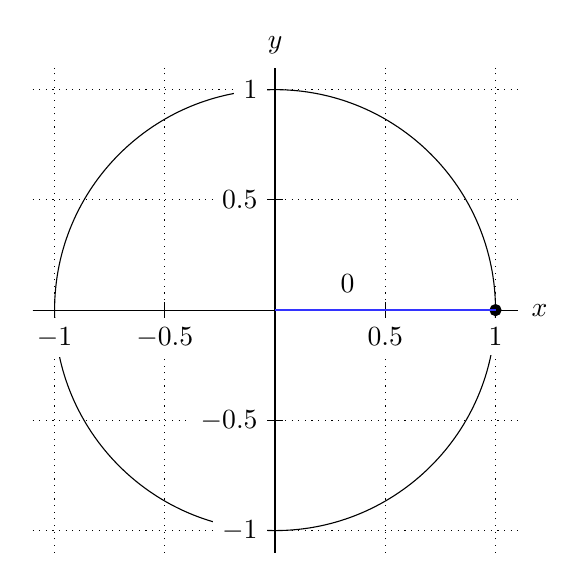
\begin{tikzpicture}[scale=2.8]
    \unitcircleAxes{0}
    \labelXAxis{-1pt}
    \labelYAxis{-1pt}
    \triangleUnitCircle{0}{0}
    \draw (20:0.35cm) node {$0$};
\end{tikzpicture}
\end{minipage}
\begin{minipage}{0.5\linewidth}
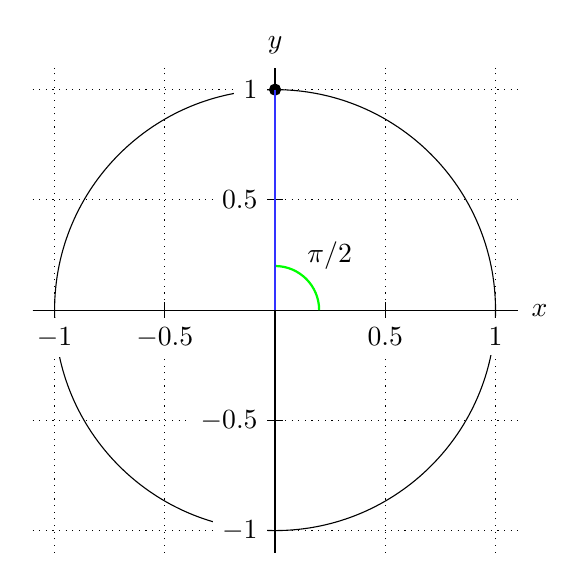
\begin{tikzpicture}[scale=2.8]
    \unitcircleAxes{90}
    \labelXAxis{-1pt}
    \labelYAxis{-1pt}
    \triangleUnitCircle{90}{-1}
    \draw (45:0.35cm) node {$\pi/2$};
\end{tikzpicture}
\end{minipage}

%\vspace{3em}

\begin{minipage}{0.5\linewidth}
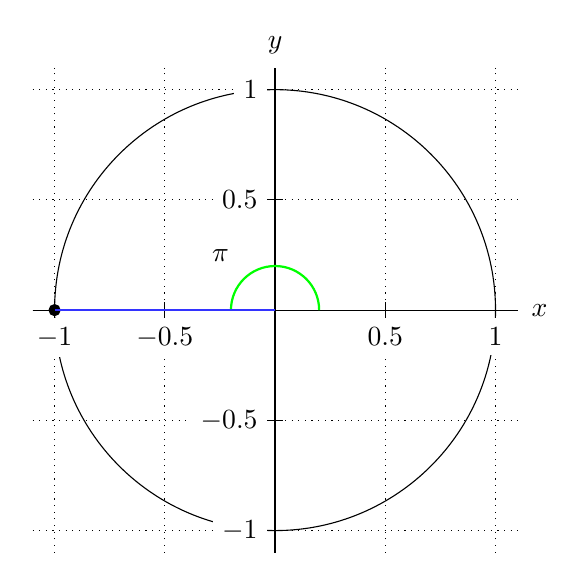
\begin{tikzpicture}[scale=2.8]
    \unitcircleAxes{180}
    \labelXAxis{-1pt}
    \labelYAxis{-1pt}
    \triangleUnitCircle{180}{0}
    \draw (135:0.35cm) node {$\pi$};
\end{tikzpicture}
\end{minipage}
\begin{minipage}{0.5\linewidth}
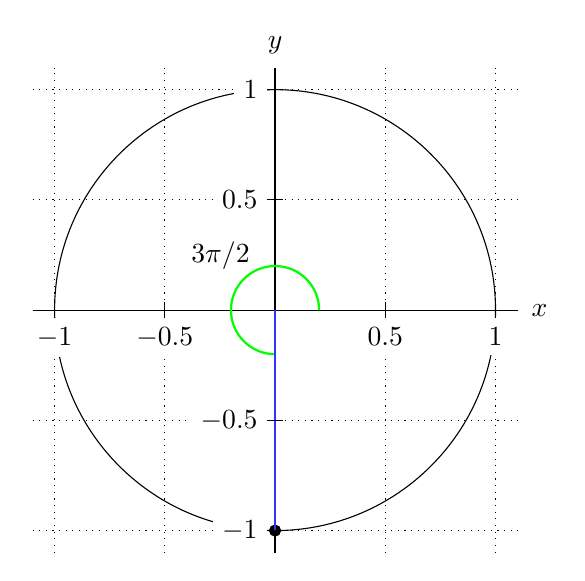
\begin{tikzpicture}[scale=2.8]
    \unitcircleAxes{270}
    \triangleUnitCircle{270}{1}
    \draw (135:0.35cm) node {$3\pi/2$};
    \labelXAxis{-1pt}
    \labelYAxis{-1pt}
\end{tikzpicture}
\end{minipage}


\begin{minipage}{0.5\linewidth}
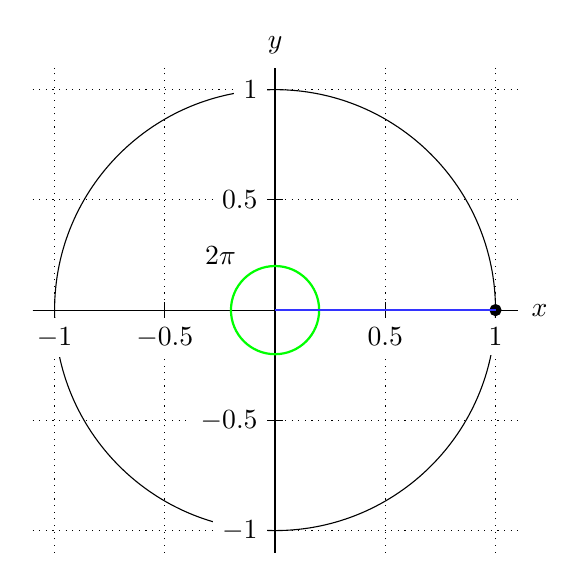
\begin{tikzpicture}[scale=2.8]
    \unitcircleAxes{360}
    \labelXAxis{-1pt}
    \labelYAxis{-1pt}
    \triangleUnitCircle{360}{0}
    \draw (135:0.35cm) node {$2\pi$};
\end{tikzpicture}
\end{minipage}


\clearpage

Angles whose reference angles are $\frac{\pi}{4}$ are aligned with the
diagonal lines from the origin. In each plot below label and define
the reference angle. Also, determine and label the sine and cosine of
the angle based on the $x$ and $y$ position of the point on the unit
circle.

\begin{minipage}{0.5\linewidth}
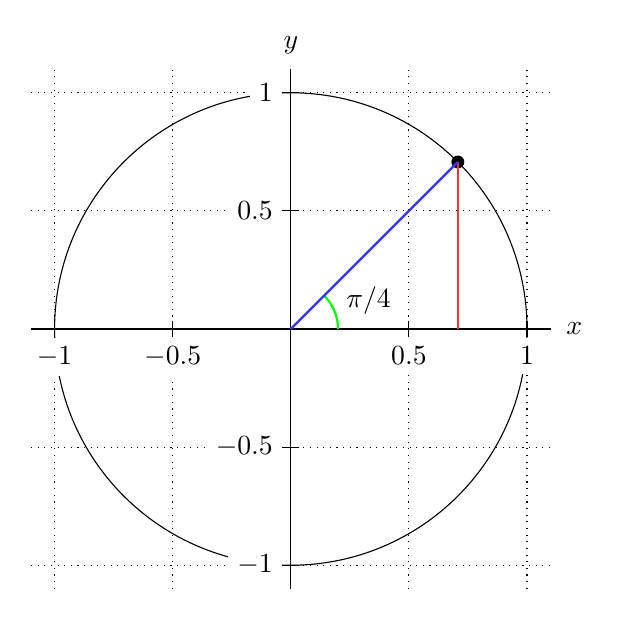
\begin{tikzpicture}[scale=3]
    \unitcircleAxes{45}
    \labelXAxis{-1pt}
    \labelYAxis{-1pt}
    \triangleUnitCircle{45}{-sqrt(2)/2}
    \draw (20:0.35cm) node {$\pi/4$};
\end{tikzpicture}
\end{minipage}
\begin{minipage}{0.5\linewidth}
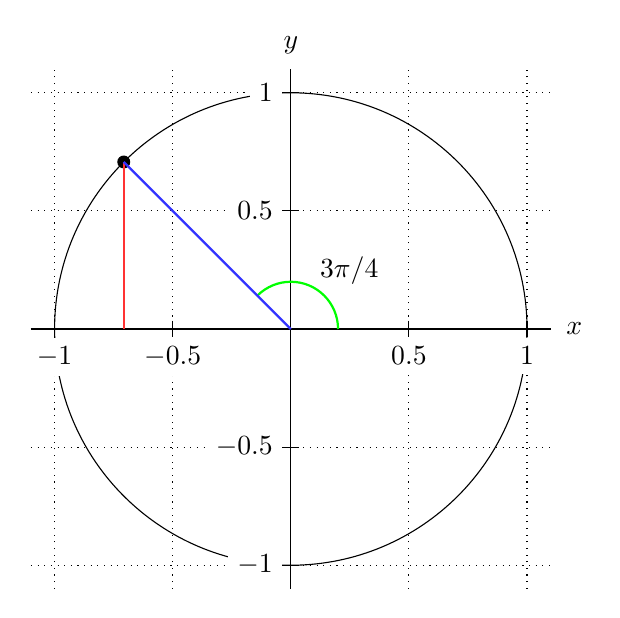
\begin{tikzpicture}[scale=3]
    \unitcircleAxes{135}
    \labelXAxis{-1pt}
    \labelYAxis{-1pt}
    \triangleUnitCircle{135}{-sqrt(2)/2}
    \draw (45:0.35cm) node {$3\pi/4$};
\end{tikzpicture}
\end{minipage}

\vspace{3em}

\begin{minipage}{0.5\linewidth}
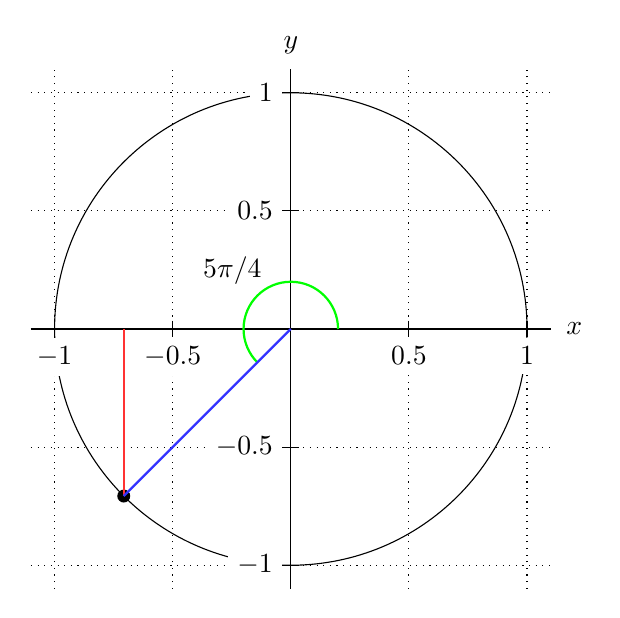
\begin{tikzpicture}[scale=3]
    \unitcircleAxes{225}
    \labelXAxis{-1pt}
    \labelYAxis{-1pt}
    \triangleUnitCircle{225}{sqrt(2)/2}
    \draw (135:0.35cm) node {$5\pi/4$};
\end{tikzpicture}
\end{minipage}
\begin{minipage}{0.5\linewidth}
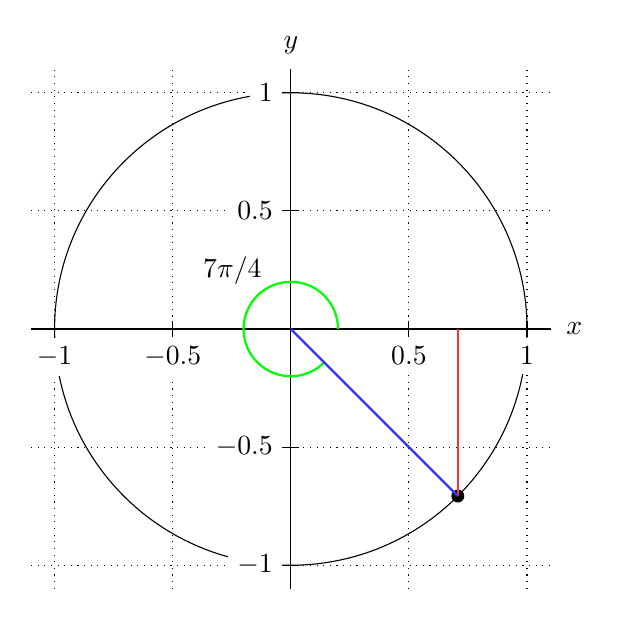
\begin{tikzpicture}[scale=3]
    \unitcircleAxes{315}
    \triangleUnitCircle{315}{sqrt(2)/2}
    \draw (135:0.35cm) node {$7\pi/4$};
    \labelXAxis{-1pt}
    \labelYAxis{-1pt}
\end{tikzpicture}
\end{minipage}

\vfill

\clearpage

Angles whose reference angles are $\frac{\pi}{6}$ have $y$ values that
are $\pm\half$. In each plot below label and define the reference
angle. Also, determine and label the sine and cosine of the angle
based on the $x$ and $y$ position of the point on the unit circle.


\begin{minipage}{0.5\linewidth}
  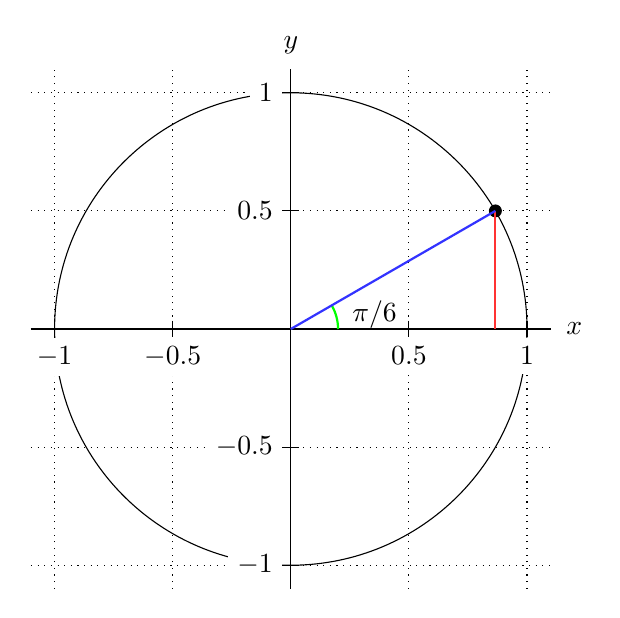
\begin{tikzpicture}[scale=3]
    \unitcircleAxes{30}
    \labelXAxis{-1pt}
    \labelYAxis{-1pt}
    \triangleUnitCircle{30}{-0.5}
    \draw (10:0.36cm) node {$\pi/6$};
  \end{tikzpicture}
\end{minipage}
\begin{minipage}{0.5\linewidth}
  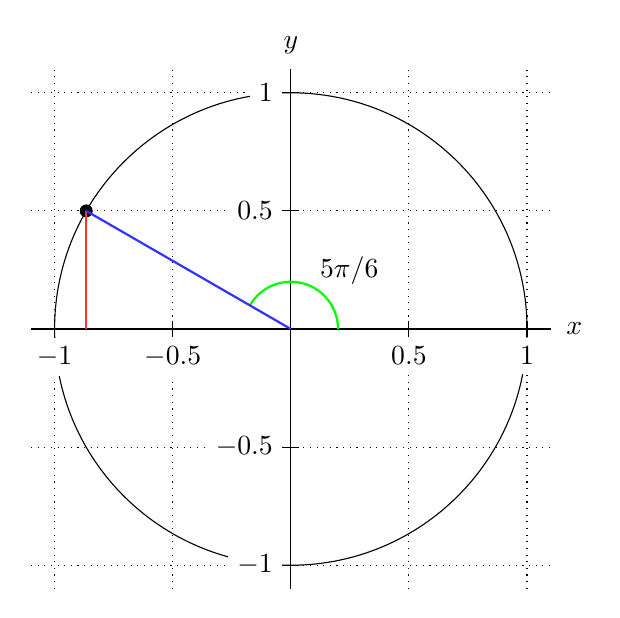
\begin{tikzpicture}[scale=3]
    \unitcircleAxes{150}
    \labelXAxis{-1pt}
    \labelYAxis{-1pt}
    \triangleUnitCircle{150}{-0.5}
    \draw (45:0.35cm) node {$5\pi/6$};
  \end{tikzpicture}
\end{minipage}


\vspace{3em}

\begin{minipage}{0.5\linewidth}
  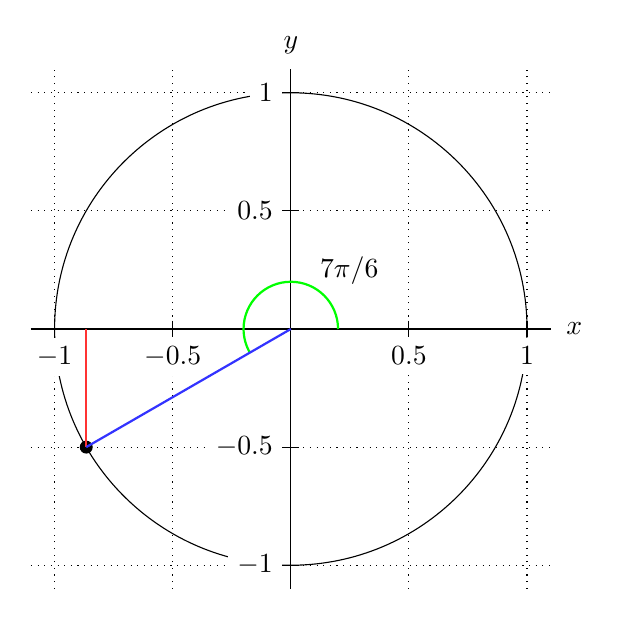
\begin{tikzpicture}[scale=3]
    \unitcircleAxes{210}
    \labelXAxis{-1pt}
    \labelYAxis{-1pt}
    \triangleUnitCircle{210}{0.5}
    \draw (45:0.35cm) node {$7\pi/6$};
  \end{tikzpicture}
\end{minipage}
\begin{minipage}{0.5\linewidth}
  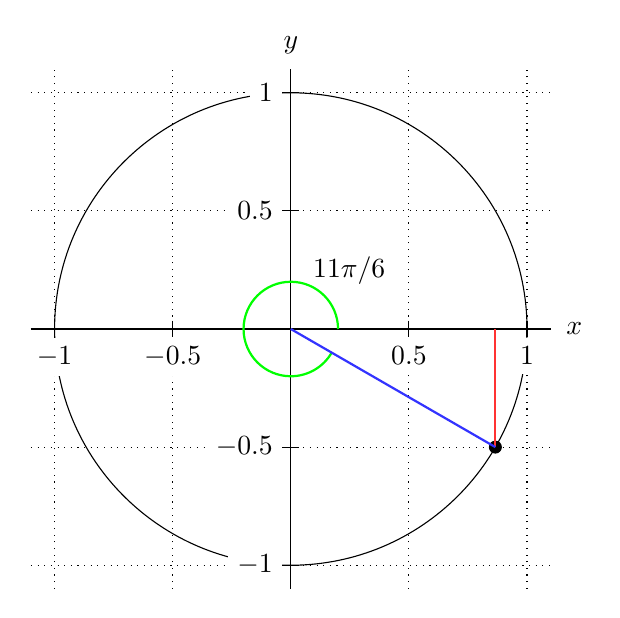
\begin{tikzpicture}[scale=3]
    \unitcircleAxes{330}
    \labelXAxis{-1pt}
    \labelYAxis{-1pt}
    \triangleUnitCircle{330}{0.5}
    \draw (45:0.35cm) node {$11\pi/6$};
  \end{tikzpicture}
\end{minipage}

\vfill

\clearpage

Angles whose reference angles are $\frac{\pi}{3}$ have $x$ values that
are $\pm\half$. In each plot below label and define the reference
angle. Also, determine and label the sine and cosine of the angle
based on the $x$ and $y$ position of the point on the unit circle.


\begin{minipage}{0.5\linewidth}
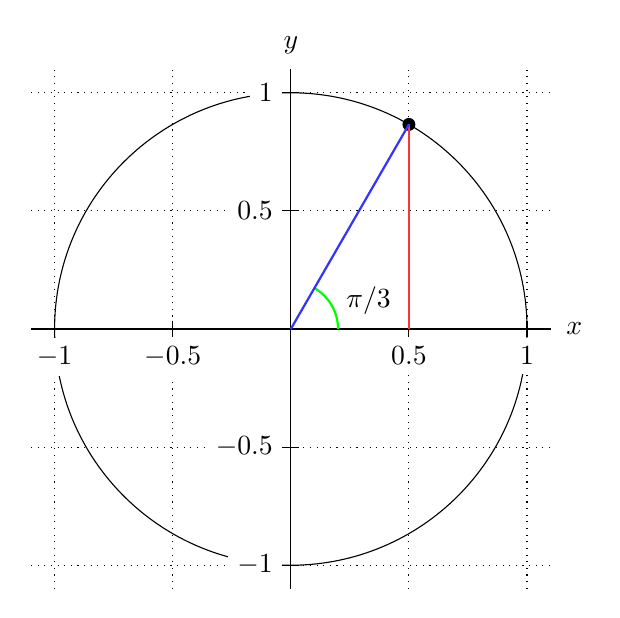
\begin{tikzpicture}[scale=3]
    \unitcircleAxes{60}
    \labelXAxis{-1pt}
    \labelYAxis{-1pt}
    \triangleUnitCircle{60}{-sqrt(3)/2}
    \draw (20:0.35cm) node {$\pi/3$};
\end{tikzpicture}
\end{minipage}
\begin{minipage}{0.5\linewidth}
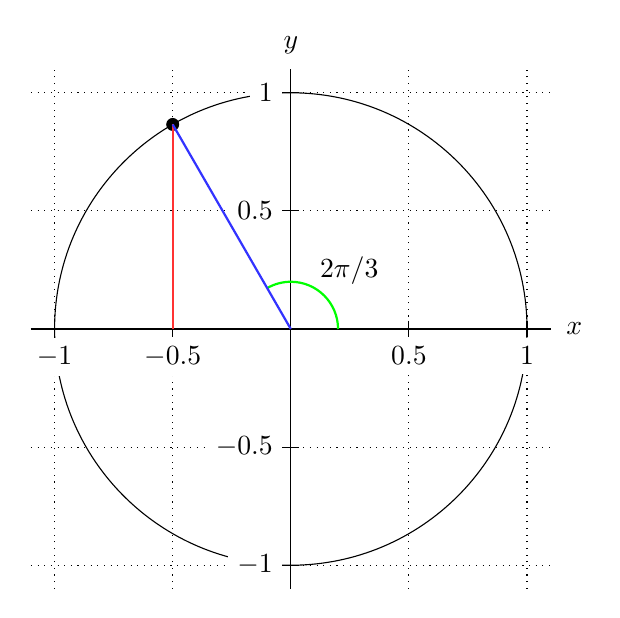
\begin{tikzpicture}[scale=3]
    \unitcircleAxes{120}
    \labelXAxis{-1pt}
    \labelYAxis{-1pt}
    \triangleUnitCircle{120}{-sqrt(3)/2}
    \draw (45:0.35cm) node {$2\pi/3$};
\end{tikzpicture}
\end{minipage}

\vspace{3em}

\begin{minipage}{0.5\linewidth}
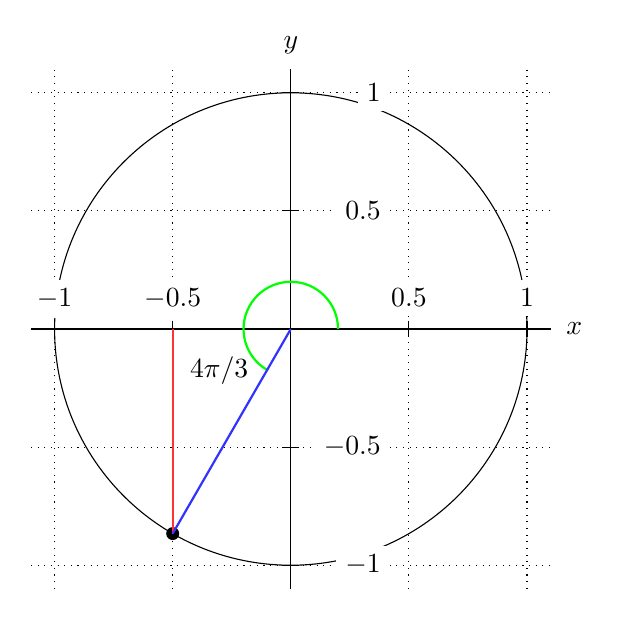
\begin{tikzpicture}[scale=3]
    \unitcircleAxes{240}
    \labelXAxis{6pt}
    \labelYAxis{12pt}
    \triangleUnitCircle{240}{sqrt(3)/2}
    \draw (210:0.35cm) node {$4\pi/3$};
\end{tikzpicture}
\end{minipage}
\begin{minipage}{0.5\linewidth}
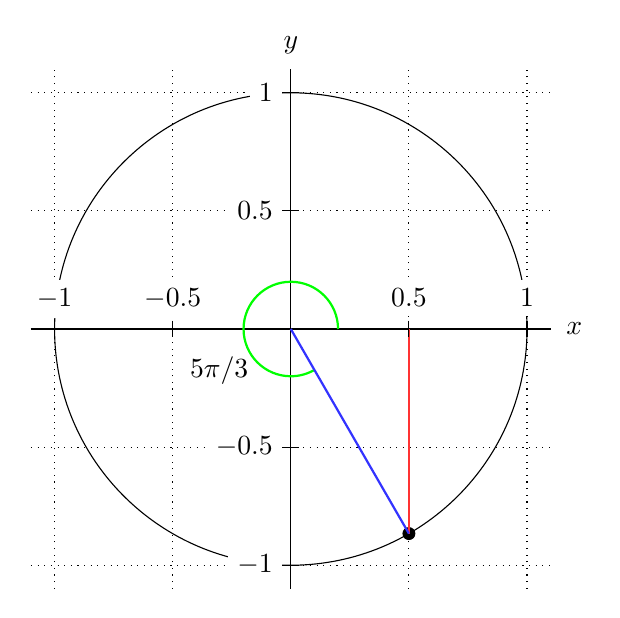
\begin{tikzpicture}[scale=3]
    \unitcircleAxes{300}
    \triangleUnitCircle{300}{sqrt(3)/2}
    \draw (210:0.35cm) node {$5\pi/3$};
    \labelXAxis{6pt}
    \labelYAxis{-1pt}
\end{tikzpicture}
\end{minipage}

\vfill

%%% Local Variables:
%%% mode: latex
%%% TeX-master: "../labManual"
%%% End:
